\chapter{Arquitetura}

\section{Introdução}
A arquitetura foi pensada para ser implementada com o Docker e Docker Compose. Cada
programa que precisa ser executado é rodado em um serviço separado. Exceto, o Guinicorn,
todos os outros serviços usaram imagens prontas do Docker Hub o que oferece mais segurança
com as atualizações constantes.

\begin{figure}[ht]
    \begin{center}
    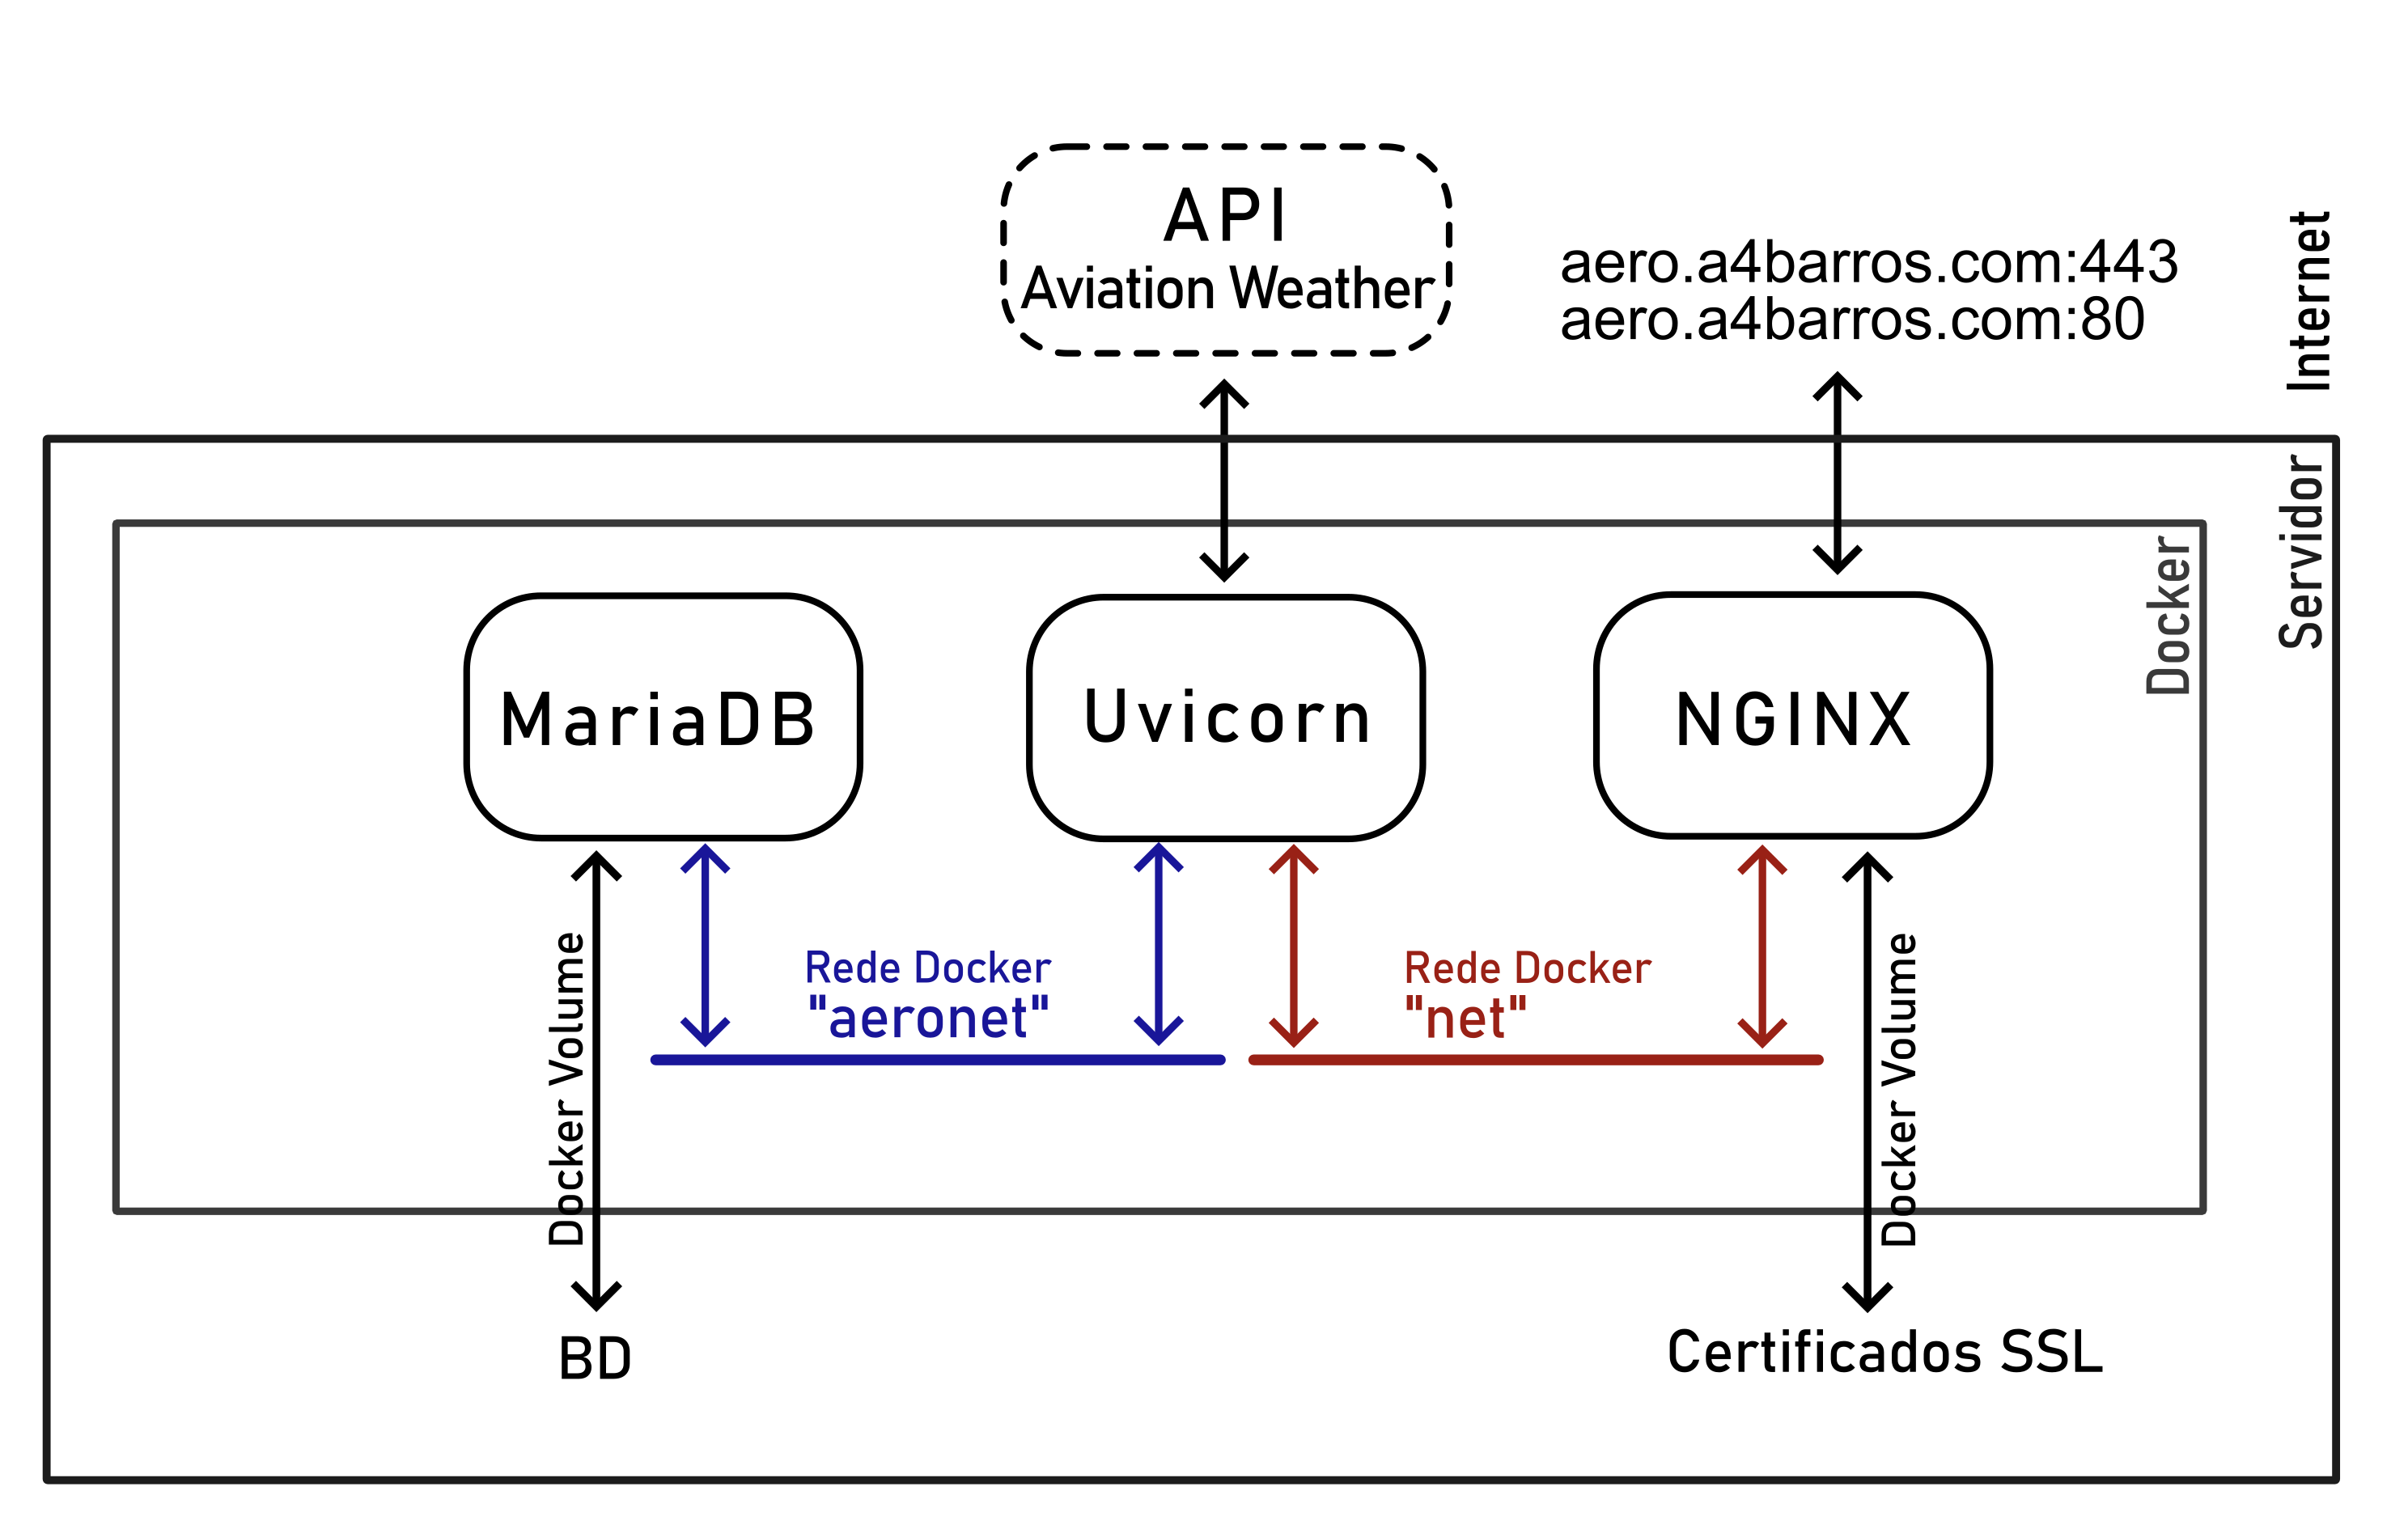
\includegraphics[width=\linewidth]{img/diagrama-arquitetura.png}
    \caption{Modelo de Arquitetura}
    \label{fig:arquitetura}
    \end{center}
\end{figure}

\section{Flask/Guinicorn}

Já que o Guinicorn é o serviço principal: o servidor onde o backend implementado em Flask roda,
fiz um Dockerfile próprio iniciando a partir de uma imagem do Alpine, devido ser lightweight.
O Python e as dependencias do projeto são instaladas automaticamente pelo Dockerfile e por
fim o arquivo de entrada \texttt{server.py} é executado usando o servidor Guinicorn. As configurações
dele ficam no arquivo \texttt{gunicorn\_config.py} é apenas configura a porta para 5000 e usa três workers.

A documentação do Guinicorn informa a seguinte fórmula para determinar a quantidade de workers. \cite{number-work}

\begin{equation} 
    \begin{split}
        N_{worker} = 2 * N_{cores} + 1 \\
        N_{worker} = 2 * 1 + 1 = 3 
    \end{split}
\end{equation}

\section{Docker Network}
A porta 5000 do Guinicorn não estará disponível para todos os serviços. Por segurança, é usada a função de
"network". Observe no diagram que a proxy NGINX compartilha com o Guinicorn a rede "net", para o NGINX,
o Guinicorn não pode ser acessado por \texttt{localhost:5000} e sim por \texttt{http://aero:5000}, "aero"
sendo o nome do serviço no Docker Compose.

Já o banco de dados em memória Redis e o banco relacional MariaDB compartilham a rede Docker "aeronet".
Apenas eles dois e o Guinicorn possuem acesso a ela, isto é necessário para que o servidor consiga ler
e escrever valores nas tabelas do banco e ler e escrever chaves-valor no Redis. Porém o NGINX não possui
acesso aos dois bancos, por mais que os bancos tenham senhas, é uma barreira a mais contra uma invasão.

\section{Docker Secrets}

Para aumentar a segurança de acesso aos dois banco é usada a função "secrets". Nela, no Docker Compose,
você informa um arquivo de texto no host onde estará uma senha, uma senha por arquivo. No mesmo Compose,
você informa quais serviços tem acesso a cada senha, na execução dos containers, as senhas são
guardadas dentro de arquivos montados no caminho "/run/secret/algum-nome.txt" em que "algum-nome" é
o mesmo nome do arquivo que estava no host.
Tanto os bancos como o servidor Guinicorn usam este método para terem acessos às senhas dos bancos.

\section{Serviços}

\subsection{MariaDB}
Este banco de dados relacional guarda toda a informação mais ou menos fixa sobre os aerodromos
conforme explicado no capítulo de modelo de dados.

\subsection{Redis}
O Redis é um banco de acesso mais rápido por estar com as informações salvas em memória em vez
de disco rígido/SSD. Ele é um espelho do que existe no banco relacional, claro que com as devidas
modificações já que o Redis possui sistema-chave valor, não sendo relacional.

\subsection{Proxy NGINX}
Faz o HTTPS funcionar, dá suporte ao HTTP/2 e ao header HTTP keep-alive. O Guinicorn só tem suporte
ao primeiro. De qualquer caso a documentação do Guinicorn não recomenda que ele esteja diretamente
ligado a Intenet \cite{nginx-gunicorn}. Já que tenho outros projetos na mesma máquina, uso subdomínios, caso o subdomínio 
seja aero.a4barros.com, o NGINX realiza uma proxy pass para a "https://aero:5000".





